\documentclass{article}

\usepackage{amsmath, amsfonts, amsthm} 
\usepackage{listings}
\usepackage{graphicx}
\usepackage{float}
\usepackage{subfigure}
\usepackage{geometry}
\usepackage{mathtools}
\usepackage{amssymb}
\usepackage{tabulary}
\usepackage{booktabs}
\usepackage{float}
\usepackage{multirow}
\usepackage{hyperref}       % hyperlinks

\geometry{
	paper=a4paper, 
	top=2.5cm,
	bottom=2.5cm, 
	left=2.5cm, 
	right=3cm,
	headsep=0.75cm, 
}
\title{Final Report}
\author{Zhuang Yulun 11811126}
\date{\today}

\begin{document}

\maketitle

\section{Problem Definition}
In this project, we are going to design a neural machine translator which translate German to English in order to gain a higher BLEU score. This project must be completed without plagiarism. We will clearly explain our algorithm and evaluate the performance of our method on the provided test dataset with BLEU evaluation metric. We will use Multi30K dataset for this task. It contains around 30,000 parallel English, German and French sentences, each with about 12 words per sentence.

To make sure that the results can be reproduced, we will explicitly set the random seeds for deterministic results. During the training, a validation set will be used to monitor the overfitting status. We will use the loss curve of our training set and validation set to evaluate the training result.

\section{Data Preparation}
Data preparation is of vital important for any kinds of Machine Learning (ML) tasks. The Multi30K dataset has $29k$ training sentences, $1k$ validation sentences and $1k$ test sentences. In training sentences, it has $18669$ and $9795$ unique words for German and English vocabulary respectively.

In our approach, we use spaCy trained tokenizer \textit{en\_core\_web\_sm} for English and \textit{de\_core\_news\_sm} for German. Our data preparation contains 5 steps.

\begin{itemize}
    \item Tokenization: break a piece of text down into a list of tokens.
    \item Building vocabulary: use a dictionary (hash table) to count word frequencies.
    \item One-Hot Encoding: use the dictionary to map words to a list of indices, so-called sequence.
    \item Batchtify: transform a dataset into mini-batches that can be processed efficiently.
    \item Sentences Aligning: pad sentences with zeros to the maximum length in one batch.
\end{itemize}

These five steps should be done for training, validation and test data.
Functions \textit{build\_vocab}, \textit{sen2tensor}, \textit{batchtify} in \textit{utils.py} are implemented for this section. 

\section{Experiments}
This section describes the training policy for our models.

\subsection{Hyperparameters}
Overall there are 9 hyperparameters (Tab.\ref{tab:table_of_notation}) affacting the model performance significantly. 


\begin{table}[H]
    \caption{Hyperparameter Notations}
    \centering % to have the caption near the table
    \label{tab:table_of_notation}
    \begin{tabular}{r c p{10cm} }
    \toprule
    $B$ & $=$ & Batch size\\
    $N_{enc}$ & $=$ & Encoder layers numbers\\
    $N_{dec}$ & $=$ & Decoder layers numbers\\
    $d_{model}$ & $=$ & Embedding dimension\\
    $d_{ff}$ & $=$ & Feedforward network dimension\\  
    $h$ & $=$ & Head numbers of multihead attention layer\\  
    $P_{drop}$ & $=$ & Dropout rate\\  
    $n$ & $=$ & Training epoch numbers\\  
    $LR$ & $=$ & Learning rate\\      
    $Fre$ & $=$ & Min frequencies of words for building vocabulary\\      
    \bottomrule
    \end{tabular}
\end{table}

\subsection{Hardware}
We trained our models on one laptop with NVIDIA GTX1060 GPU and one GPU server with NVIDIA GTX2080 GPU respectively. For our average models using $10M-50M$ parameters, each training epoch took about 60 seconds on laptop and 30 seconds on GPU server. We trained the base models for a total of 40 epochs. 

\subsection{Training Setup}
We design our loss function, optimizer and regularization to be as close as those described by \textit{Ashish et al}\cite{vaswani2017attention}. However, we design our learning rate to be a constant, which was proven to be more efficient than a noam decay function\cite{devlin2018bert}.

\begin{table}[H]\caption{Training Setup}
    \centering % to have the caption near the table
    \begin{tabular}{r c p{10cm} }
    \toprule
    $Loss\ Function$ && \textit{nn.CrossEntropyLoss}\\
    $Optimizer$ && \textit{optim.Adam} with $\beta_1=0.9$, $\beta_2=0.98$ and $\epsilon=10^{-9}$\\
    $Regularization$ && \textit{nn.Dropout} and \textit{nn.LayerNorm}.\\
    \bottomrule
    \end{tabular}
    \label{tab:table_of_setup}
\end{table}

\section{Results}
The highest BLEU score for our model is $37.14$.

% Discuss how and why different choices influenced your performance (Important)
\subsection{Model Evaluation and BLEU Scores}

We use training loss and validation loss to evaluate our models directly. We observe that transformer with the half size parameters as described by \textit{Ashish et al}\cite{vaswani2017attention} will perform best.
As required for compotetion purpose, we also use Bilingual Evaluation Understudy (BLEU) as our evaluation metric. BLEU has been a de-facto standard for evaluating translation outputs since it was first proposed in 2002. We compute the BLEU score of our de-en model with the $multi-bleu.perl$ \href{https://github.com/moses-smt/mosesdecoder/blob/master/scripts/generic/multi-bleu.perl}{script}.

Since our models are training on a quite small dataset , overfitting becomes the most troublesome challenge shown in Fig.\ref{fig: overfit}.

\begin{figure}[H]
    \centering
    \subfigure[Overfitting at $val\_loss \approx 2$]{
        \textsf{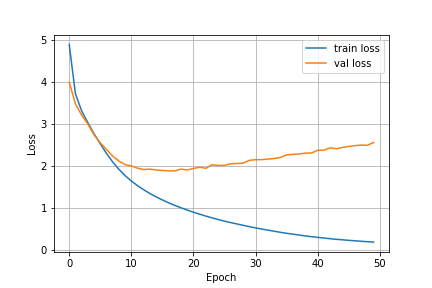
\includegraphics[width=0.4\columnwidth]{figs/transformer-5-19-base.png}}
    }
    \quad
    \subfigure[Overfitting at $val\_loss \approx 1.5$]{
        \textsf{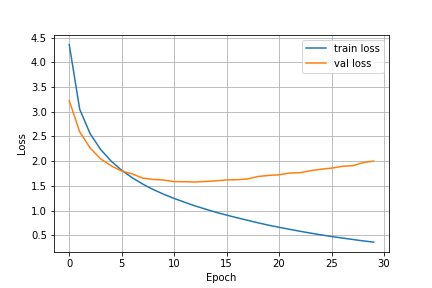
\includegraphics[width=0.4\columnwidth]{figs/transformer-5-19-base2.png}}
    }
    \caption{Overfitting training and validation loss curves}
    \label{fig: overfit}
\end{figure}


\subsection{Hyper-Parameters Tuning}

In this project, we have tuned a large set of hyperparameters to gain a higher BLEU score from transformer. As shown in Table \ref{tab:tuning}, models named with full data were trained on our local laptop and those named with partial data were trained on a GPU server. 

To evaluate the importance of different components of the Transformer, we varied our model in different ways. We found that BLEU drops off with too many heads but BLEU stay unchanged from 4 to 8.
In Table \ref{tab:tuning} rows 1 to 4, we vary the embedding size from 512 to 1024 and encountered great overfitting due to the large number of embedding layer parameters.
We further observe in rows 11 and 11 that, not as expected, bigger models are not better, and dropout is very helpful in avoiding over-fitting.

We have also encountered two strange evidences.
Due to the difference of PyTorch version, we get different vocabulary size from laptop to server with same code. That is to say, the model we trained on server can not be evaluated on local laptop. 
Another strange point is that BLEU score keep raising as the min frequencies of words for building vocabulary increasing. As $min\_fre$ increasing from 1 to 3, the highest BLEU scores raising from 34.36 to 37.14.

\begin{table}[H]
    \caption{Hyperparameter Tuning}
    \centering % to have the caption near the table
    \label{tab:tuning}
    \begin{tabular}{c|c|cccccccc}
    \hline
    \textbf{$Model$} & \textbf{$BLEU$} & \textbf{$Loss$} & \textbf{$Fre$} & \textbf{$N_{enc}$} & \textbf{$N_{dec}$} & \textbf{$d_{model}$} & \textbf{$d_{ff}$} & \textbf{$P_{drop}$} & \textbf{$B$} \\ \hline
    5-18 & 33.13 &  & 1 & 3 & 3 & 512 & 512 & 0.1 & 128 \\
    5-19-0.5 & 34.36 &  & 1 & 3 & 3 & 512 & 512 & 0.5 & 128 \\
    5-19 & 28.77 &  & 1 & 4 & 4 & 512 & 512 & 0.1 & 128 \\
    5-19-base & 29.16 &  & 1 & 6 & 6 & 512 & 1024 & 0.1 & 64 \\
    5-19-base2 & 35.7 &  & 2 & 3 & 3 & 512 & 1024 & 0.1 & 64 \\
    5-20-1 & 30.64 &  & 2 & 3 & 3 & 256 & 512 & 0.3 & 256 \\
    5-20-2 & 30.29 &  & 1 & 3 & 3 & 256 & 512 & 0.2 & 256 \\
    5-20-3 & 34.61 &  & 1 & 3 & 3 & 512 & 2048 & 0.3 & 64 \\
    5-20-4 &  &  & 1 & 3 & 3 & 256 & 512 & 0.1 & 128 \\ \hline
    21-7 & 32.86 & 1.843 & 1 & 3 & 3 & 512 & 1024 & 0.2 & 128 \\
    21-6 & 36.06 & 1.617 & 2 & 3 & 3 & 256 & 256 & 0.1 & 256 \\
    21-8 & 34.57 & 1.589 & 2 & 3 & 3 & 256 & 512 & 0.1 & 128 \\
    21-9 & 33.69 & 1.849 & 1 & 3 & 3 & 512 & 512 & 0.1 & 128 \\
    my-21-11 &  & fail & 1 & 3 & 3 & 512 & 512 & 0.1 & 128 \\
    my-21-11 &  & fail & 1 & 3 & 3 & 512 & 512 & 0.3 & 128 \\
    21-11(layernorm) & 31.78 & 1.79 & 1 & 2 & 2 & 512 & 1024 & 0.1 & 128 \\
    21-11(layernorm) & 33.28 & 1.848 & 1 & 2 & 2 & 512 & 2048 & 0.2 & 256 \\ \hline
    6-5-1-best & 37.14 &  & 3 & 3 & 3 & 256 & 512 & 0.1 & 128 \\ \hline
    \end{tabular}
\end{table}
\subsection{Translation Results}
In this section, we implemented two translation algorithms, greedy search and beam search. 
Greedy Search algorithm selects one best candidate as an input sequence for each time step. Choosing just one best candidate might be suitable for the current time step, but when we construct the full sentence, it may be a sub-optimal choice.
The beam search algorithm selects $k$ (beam width) alternatives for an input sequence at each timestep based on conditional probability. At each time step, the beam search selects $k$ number of best alternatives with the highest probability as the most likely possible choices for the time step.
Superisingly the changing range of BLEU is within 0.2. The sample translation sentences are shown in Table \ref{t:sample}.


\begin{table*}[h]
    \centering
    \begin{tabular}{c|p{15cm}}
    \multicolumn{2}{c}{{\bf German-English translations}}\\
      \hline
    src & In einem Interview sagte Bloom jedoch , dass er und Kerr sich noch immer lieben . \\
      \hline
    ref & However , in an interview , Bloom has said that he and \textit{Kerr} still love each other . \\
      \hline
    {\it best} & In an interview , however , Bloom said that he and \textit{Kerr} still love . \\
      \hline
    base & However , in an interview , Bloom said that he and \textbf{Tina} were still $<$unk$>$ . \\
      \hline
      \hline
    src & Wegen der von Berlin und der Europ \\ 
      \hline
    ref & The imposed on national economies through adherence to the common currency , has led many people to think Project Europe has gone too far .\\
      \hline
    {\it best} & Because of the strict 
    respective national economy is forced to adhere to the common currency , many
    people believe that the European project has gone too far . \\
      \hline
    base & Because of the pressure ct has gone too far .\\
    \end{tabular}
    \caption{{\bf Sample translations} -- %examples in both translation directions.
    for each example, we show the source ({\it src}), the human translation ({\it
    ref}), the translation from our best model ({\it best}), and the
    translation of a non-attentional model ({\it base}).  We italicize some
    \textit{correct} translation segments and highlight a few \textbf{wrong} ones in
    bold.} % See Appendix~\ref{sec:sample} for detailed descriptions.}
    \label{t:sample}
\end{table*}

\end{document}
